\documentclass{article}
\usepackage[utf8]{inputenc}
\title{Lecture 4:SVM}
\author{wbg231 }
\date{December 2022}
\newcommand{\R}{$\mathbb{R}$}
\newcommand{\B}{$\beta$}
\newcommand{\A}{$\alpha$}
\newcommand{\D}{\Delta}

\newcommand{\avector}[2]{(#1_2,\ldots,#1_{#2})}
\newcommand{\makedef}[2]{$\textbf{#1}$:#2 }
\usepackage{tikz,graphicx,hyperref,amsmath,amsfonts,amscd,amssymb,bm,cite,epsfig,epsf,url}

\begin{document}

\maketitle

\section*{introduction}
\begin{itemize}
\item \href{https://nyu-ds1003.github.io/mlcourse/2023/lectures/lec04/04.pdf}{slides}
\section{maximum margin classifier}
\subsection{linearly separable data }
\item 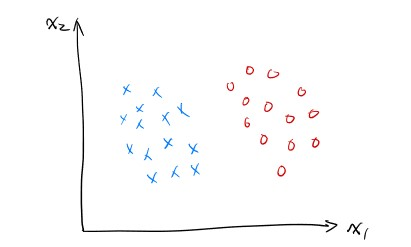
\includegraphics[width=10cm]{lecture_notes/lecture_4/immmages/l4_1.jpg}
\item suppose we have a dataset that looks like the above with two classes red and blue that are represented as -1,1
\item how could we fine a hyperplane to separate the classes.
\item specifically we want 
\begin{itemize}
    \item consider $w$ which is a vector normal (orthogonal) to the hyperplane 

    
    \item $w^{t}x_i>0\quad \forall i \text{ s t }y_i=1 $
    \item $w^{t}x_i<0\quad \forall i \text{ s t }y_i=-1 $ 
    \item so notice this means that first of all $w^{t}x=<w,x>=0\rightarrow$ x is on the hyperplane since w is orthogonal to the hyperplane
    \item so if a point $w^{t}x_i>0$ it means that the angle between a vector orthogonal to the hyper plane and that $x_i$ is greater than 90, meaning that point is on the left side of the hyperplane 
  \item   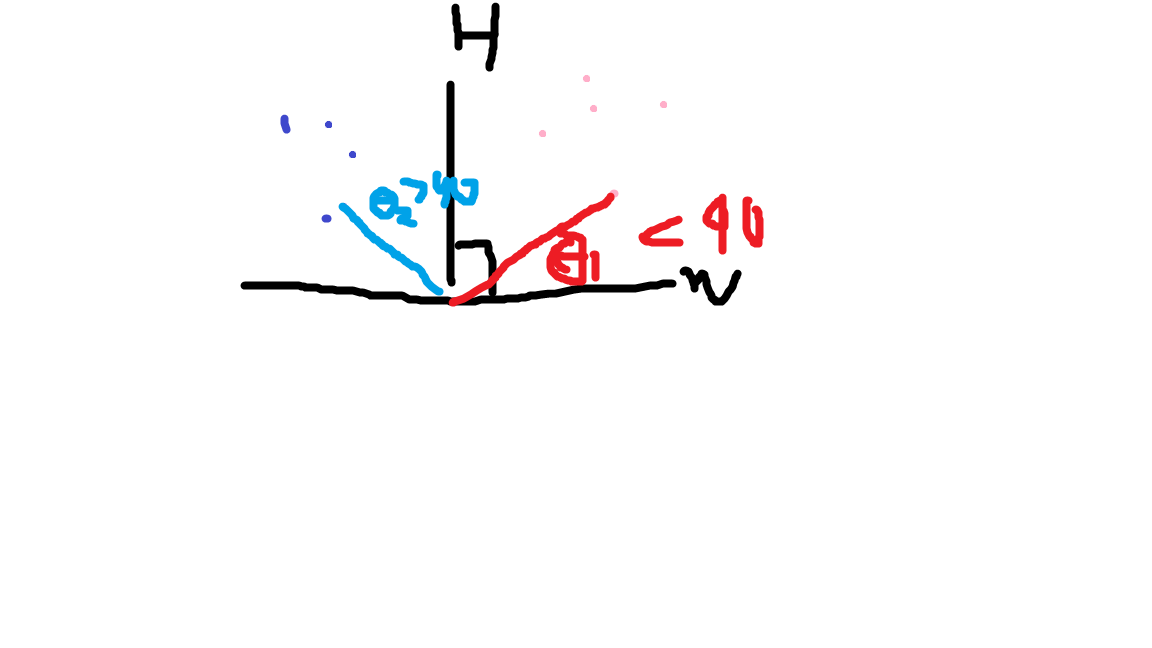
\includegraphics[width=10cm]{lecture_notes/lecture_4/immmages/l4_2.png}
    \item image our hyper plane h is the y axis, and w is the x axis. 
    \item the pink points are on the right side of the y axis and thus the angle between them$\theta_{1}<90$
\end{itemize}
\item so what this is really saying is we can find a hyperplane that will perfectly separate our data 
\subsection{the perception algorithm}
\item algo
\begin{itemize}
    \item initialize $w\leftarrow 0$
    \item while there are still miss classifications 
    \begin{itemize}
        \item for $(x_i,y_i)\in\mathcal{D}$
        \begin{itemize}
            \item if $y_iw^tx_i<0$ (ie we miss classify a point)
            \item $w \leftarrow w+y_ix_i$ we move our w in the other direction 
        \end{itemize}
    \end{itemize}
\end{itemize}
    \item basically until we miss classify no data points, loop through our dataset and everywhere we miss classify a data point shift our w slightly in ta ht direction 
    \item in other words move towards miss classified positive examples (ie make the angle smaller) and away from negative examples (make the angle larger)
    \item this is guaranteed to find a classifier with zero error if one exists 
    \item if we think of this as gradient descent it is more or less $\ell(w)=-y_iw^{t}x_i$ note that $y_i$ is a real number. thus we have $\nabla \ell(w)=-y_ix_i$
    meaning our update rule is $w\leftarrow w+y_ix_i$
\subsection{maximum margin separating hyperplane}
\item 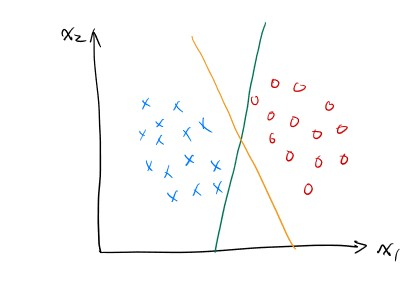
\includegraphics[width=10cm]{lecture_notes/lecture_4/immmages/l4_3.jpg}
\item linearly separable data could have infinite hype planes that separate it with zero loss (that is the perception solution is not unique
\item which one do we pick?
\item we prefer the classifier that is furthest away from both classes
\item think of the geometric margin as the smallest distance between the hyperplane and the points 
\item the maximum margin is the largest distance between the nearest point in each class
\subsection{geometric margin}
\item our goal is to maximise the distance between the separating hyperplane and the closest points we can formalize this  
\item we say $(x_i,y_i)$ for $i\in[1,n]$ are linearly separable if there is a $w\in\mathbb{R}^{d}$ and $b\in \mathbb{R}$ such that $y_i(w^{t}x_i+b)>0\quad \forall i$ the set $\{v \in\mathbb{R}^{d}|w^{t}b+b=0\}$ is called the separating hyperplane 
\item so to break that down in 2d $\{v \in\mathbb{R}^{d}|w^{t}b+b=0\}$ defines a line that is shifted by b and thus  does not need to pass through the origin. and has $w$ orthogonal to it everywhere. 
\item then we have $(w^{t}x_i)+b$ is the sign of the correct sign of the hyper plane $y_i(w^{t}x_i)+b)>0$ just means we have all classifications correct
\item let H be a hyperplane that separates data $(x_i,y_i)\quad \forall i$ the geometric margin of this hyperplane is $$min_{i}d(x_i,H)$$ where d is the distance to the hyperplane, that is the distance to the nearest point. 
\subsection{distance between a point and hyperplane}
\item so recall that the projection of $v\in\mathbb{R}^{d}$ onto $w\in\mathbb{R}^{d}$ is $\frac{<v,w>}{||w||_{2}}$
\begin{itemize}
    \item i am going to quickly derive the distance between a hyperplane and point 
    \item  let x be the point and let h be the projection of x onto the hyper lane H (which is the closest point on the hyperplane to x)
    \item $d(x,h)=|x-h|$ so notice that h is the projection of x onto the hyperplane thus x-h is orthogonal to h. meaning that x-h is parallel to w ie we can express it as $x-h=\lambda w$ and thus $h=x-\lambda w$
    \item since h is on the hyper plane we know $<w,h>+b=0$ by definition and thus $<w,x-\lambda w>+b=0$
    \item this means that $<w,x>-\lambda<w,w>+b=w^{t}x-\lambda||w||_{2}^{2}+b=0$
    \item then we an solve for $\lambda$ as $\lambda=\frac{w^{t}x_i+b}{||w||_{2}^{2}}$
    \item so recall that $d(x,h)=||x-h||_{2}=||=||\lambda w||=|\lambda| ||w||=|\frac{w^{t}x+b}{||w||_{2}}|$
\end{itemize}
\item then as we are assuming H is a linearly sepearting hyper plane for the data this must hold $y_i(w^{t}x_i+b)>0$  so  we can write 
\item $d(x_i,H)=|\frac{w^{t}x_i+b}{||w||_2}|=\frac{y_{i}(w^tx_i+b)}{||w||_{2}}$
\subsection{maximising the margin}
\item so our goal is to maximise the distance between the the dataset and the hyperplane, ie max the geometric margin that is $$max (min_{i}d(x_i,H))$$
\item so that is given a hyperplane $H=\{v|w^{t}v+b=0\}$ we have $$max(min_{i}\frac{y_{i}(w^{t}x_i+b)}{||w||_{2}})$$
\item this can be rewritten trivially as $max\quad M $ subject to $\frac{y_{i}(w^{t}x_i+b)}{||w||_{2}}\geq m\quad \forall i$
\item the solution to this is still not necessarily unique as we are not restricting the length of $w$
\item to change this we can fix require that $||W||_{2}=\frac{1}{m}$
\item this allows us to re write the problem as $max m= max \frac{1}{||w||_{2}}$ subject to $\frac{y_{i}(w^{t}x_i+b)}{||w||_{2}}\geq m\Rightarrow \frac{y_{i}(w^{t}x_i+b)}{||w||_{2}}\geq \frac{1}{||w||_{2}}$ and finally $max \frac{1}{||w||_{2}}$ subject to $yi(w^{t}x_i+b)\geq 1$
\item this is equiv lent to min$\frac{1}{2}||w||_{2}^{2}$ subject to $yi(w^{t}x_i+b)\geq 1\quad \forall i$ this works because our norm is always postive, and so  $argmax_w||w||=argmax_w||w||^2$
\item so this finds the maximum norm solution that has a margin of at least 1 on all examples
\item $y_{i}(w^{t}x_i+b)$ is called the functional margin 
\subsection{soft margin SVM}
\item if the data is not linearly separable then for any w there will be points with a negative margin 
\item we can thus introduce slack variables to penalize a small margin 
\item so soft margin svm can be expressed as \\minimize $\frac{1}{2}||w||_{2}^{2}+\frac{c}{n}\Sigma_{i=1}^{n}\epsilon_{i}$       subject to $yi(w^{t}x_i+b)\geq 1-\epsilon_{i}\quad \epsilon_{i}\geq 0\quad \forall i$
\item if $\epsilon_{i}=0\quad\forall i$ then it is hard margin svm 
\item $\epsilon_{i}\geq 0$ means that certain data point will be miss classified at our decision rule 
\item c controls how much we penalize miss classifications 
\item for soft margin csv we see we can write $d(x_i,H)=\frac{y_{i}(w^{t}x_i+b)}{||w||_{2}}\geq \frac{1-\epsilon_{i}}{||w||_{2}}$ thus $\epsilon_{i}$ measures the violations by multiples of the geometric margin 
\item if $\epsilon_{i}=1$ then $x_i$ lies on the hyper plane 
\item if $\epsilon_{i}=3$ then $x_i$ we can write $1-\epsilon_{i}=-2\leq y_{i}(w^{t}x_i+b)$ while the ideal constraint is $1\leq y_{i}(w^{t}x_i+b)$ meaning that $x_i$ is 2 past 2 times the margin with beyond the learned decision  border (hyperplane )
\item 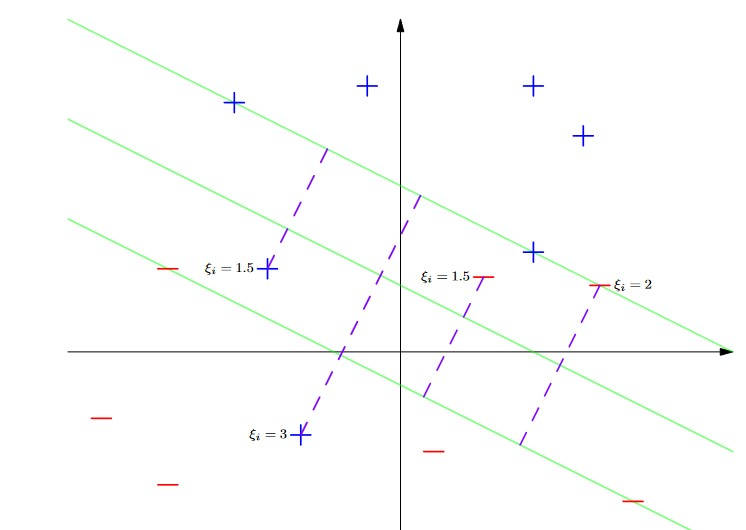
\includegraphics[width=10cm]{lecture_notes/lecture_4/immmages/l4_4.jpg}
\section{minimize the hinge loss}
\item we can also derive the SVM problem using hinge loss and ERM 
\subsection{perceptron loss}
\item the loss function of the perceptron  is $\ell(x,y,w)=max(0,-yw^{t}x)$
\item 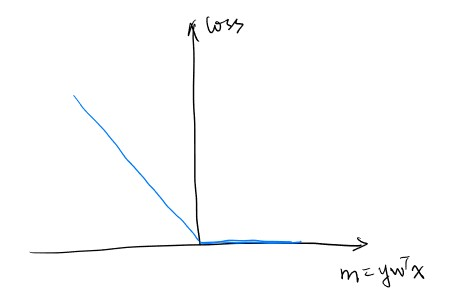
\includegraphics[width=10cm]{lecture_notes/lecture_4/immmages/l4_5.jpg}
\item notice that this is not differentiable but it is convex 
\item also if we do erm. we have $\hat{R}(w)=\frac{1}{n}\Sigma_{i=1}^{n}\ell(f(x_i),y_i)=\frac{1}{n}\Sigma_{i=1}^{n}max(0,-y_iw^tx_i)$ this does not give a unique max, any function that gets all training points right is considered perfect
\subsection{hinge loss}
\item hinge loss can be expressed as $\ell_{hinge}=max(1-m,0)=(1-m)_{+}$ ie just the positive part of 1-m
\item the margin $m=yf(x)$ 
\item the positive part $(x)_{+}=x1(x\geq 0)$
\item hinge is a convex upper bound on 0-1 loss, but it is not differentiable at m=1
\item the interpretation is we have a margin error when $m<1$
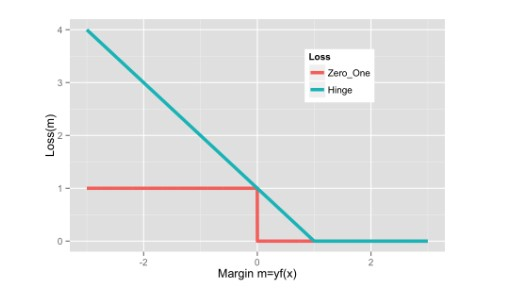
\includegraphics[width=10cm]{lecture_notes/lecture_4/immmages/l4_6.jpg}
\item zero one error is not convex
\subsection{SVM ERM}
\item using erm we can write the SVM problem 
\item our hypothesis space is $\mathcal{F}=\{f(x)=w^{t}x+b|w\in \mathbb{R}^{d}, b\in \mathbb{R}\}$ is our hypothesis space is all hyper planes in the dimension of our input data  
\item  loss= hinge loss $\ell_{hinge}=mas(1-m,0)=(1-m)_{+}$
\item so we can think of our erm in general as erm$=argmin\frac{1}{n}\Sigma_{i=1}^{n}\ell(f(x_i,y_i)x_i)$ and thus in this case we have erm=erm$=argmin_{w\in \mathbb{R}^{D},\mathbb{R}}\frac{1}{n}\Sigma_{i=1}^{n}max(0,1-y_i(w^{t}x_i+b))$ 
\item then we can make this penalized erm by adding an $l_2$ constraint as erm$=argmin_{w\in \mathbb{R}^{D},\mathbb{R}}\frac{1}{n}\Sigma_{i=1}^{n}max(0,1-y_i(w^{t}x_i+b))+\lambda||w||_{2}^{2}=argmin_{w\in \mathbb{R}^{D},\mathbb{R}}\lambda||w||_{2}^{2}+ \frac{1}{n}\Sigma_{i=1}^{n}max(0,1-y_i(w^{t}x_i+b))$ then if we set $\lambda=\frac{1}{2}$ and multiply our loss by the constant $c$ we get $argmin_{w\in \mathbb{R}^{D},\mathbb{R}}\frac{1}{2}||w||_{2}^{2}+ \frac{c}{n}\Sigma_{i=1}^{n}max(0,1-y_i(w^{t}x_i+b))$ which is exactly what we say above. 
\item this is not differentiable because of the max function 
\item we can also write this as a constrained erm as $$min \frac{1}{2}||W||^{2}+\frac{c}{m}\Sigma_{i=1}^{n}\epsilon_{i}$$ \\ $$\text{subject to } \epsilon_{i}\geq max(0,1-y_{i}[w^{y}x_i+b)\quad \forall i$$
\item and further as min $\frac{1}{2}||w||^{w}+\frac{c}{n}\sum_{i}^{n}\epsilon_{i}$ subject to $\epsilon_{i}\geq (1-y_{i}[w^{y}x_i+n], \epsilon_{i}\geq 0 \quad \forall i $
\section{sub gradient descent motivation}
\item now that we know the objective can we use stochastic gradient descent on it? 
\item no the objective is not differentiable everywhere, so we need to use sub gradient descent which generalizes gradient descent for non differential convex functions 
\subsection{SVM optimization}
\item the svm objective function with l2 regularization is $J(w)=\frac{1}{n}\Sigma_{i=1}^{n}max(0,1-y_{i}w^{t}x_{i})+\lambda||2||^{2}$
\item this is non differentiable but if there were a gradient we could express it as $\nabla _{W}j(w)=\nabla_{W}(\frac{1}{n}\Sigma_{i=1}^{n}\ell(y_iw^{t}x_i)+\lambda||w||^{2})=\frac{1}{n}\Sigma_{i=1}^{n}\nabla_{w}\ell(y_iw^{t}x_i)+2\lambda w$
\subsection{gradient of svm objective}
\item the derivative of hinge loss $\ell_{hinge}=max(0,1-m)$ is 0if $m>1 $ -1 if $m<1$ and undefined if $m=1$
\item so by the chain rule we have $\nabla_{W}\ell(y_iw^{t}x_i)=\ell^{'}(y_iw^{t}x_i)w_ix_i$ 
\item so that is 0 if $y_{i}w^{y}x_i>1$ -1 $-y_{i}x_{i}$ if $y_{i}w^{y}x_i<1$ and undefined if $y_{i}w^{y}x_i>1=0$
\item we can plug this back into our gradient equation to get \\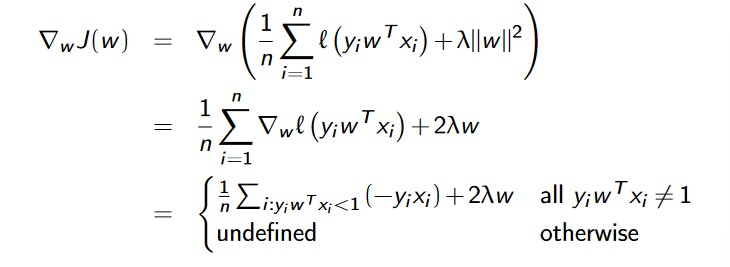
\includegraphics[width=10cm]{lecture_notes/lecture_4/immmages/l4_7.jpg}
\item so the points we get right don't factor into it only those we miss classify
\item so how do we deal with this point of non-dependability
\section{sub gradients}
\subsection{first order conditions for convex differentiable functions}
\item suppose $f: \mathbb{R}^{d}\rightarrow \mathbb{R}$ is convex and differentiable then for any x,y we will have $$f(y)\geq f(x)+\nablaf(X)^{t}(y-x)$$
\item that is the linear approximation using a first order tailor series is a global understate of f ie under the function value 
\item this also implies that $\nabla f(x)=0$ means that x is a global minimize of f
\item 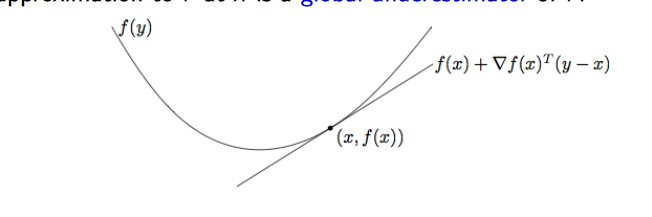
\includegraphics[width=10cm]{lecture_notes/lecture_4/immmages/l4_8.jpg}
\subsection{sub gradients}
\item a vector $g\in \mathbb{R}^{d}$ is a sub gradient of a convex function $f:\mathbb{R}^{d}\rightarrow \mathbb{R}$ at x if for all z $$f(z)\geq g^{t}(z-x)$$
\item so g just needs to be a constant, such that the function value at x + that constant time z-x is always bellow the function it is pretty much the same as a first order Taylor expansion except broader
\item \item 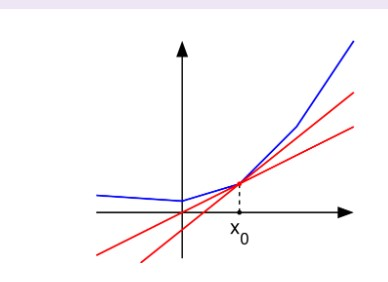
\includegraphics[width=10cm]{lecture_notes/lecture_4/immmages/l4_9.jpg}
\item notice that it does not have to unique 
\subsection{pretties}
\item the set of all sub gradients at x is called the sub differential $\partial f(x)$
\item f is a sub-differentiable at x if $\exists$ at least 1 sub gradient  at x.
\item for convex functions
\begin{itemize}
    \item f is differentiable  at x $\iff \partialf(x)=\{\nabla f(x)\}$
    \item the sub differential is always non empty 
    \item x is the global opt $\iff 0\in \partial f(x)$
\end{itemize}
\itme for non convex functions the sub differential may be an empty set, ie there may be no global underestimate 
\subsection{sub differential of the absolute value}
\item consider f(x)=$|x|$
\item the plot on the right shows $\{(x,g)|x\in\mathbb{R}, g\in \partial f(X)\}$
\item 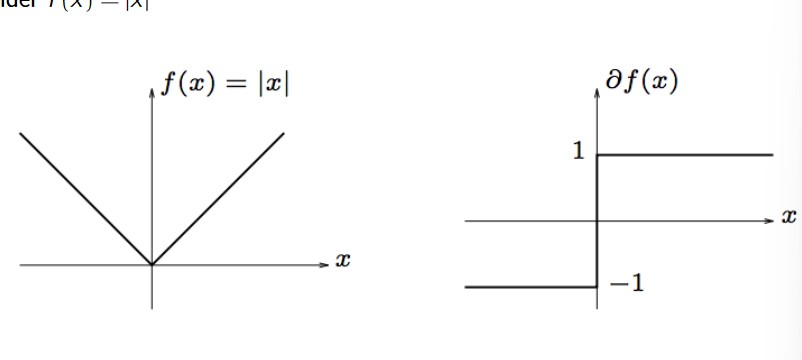
\includegraphics[width=10cm]{lecture_notes/lecture_4/immmages/l4_10.jpg}
\subsection{sub gradient example}
\item lets find the sub gradient of $f(x_1,x_2)=|x1|+2|x_2|$ at (3,0)
\item the first coordinate of the sub gradient must be 1 as the derivative of the absolute value for positive functions is 1 
\item the second coordinate can Be anything in [-2,2]
\item 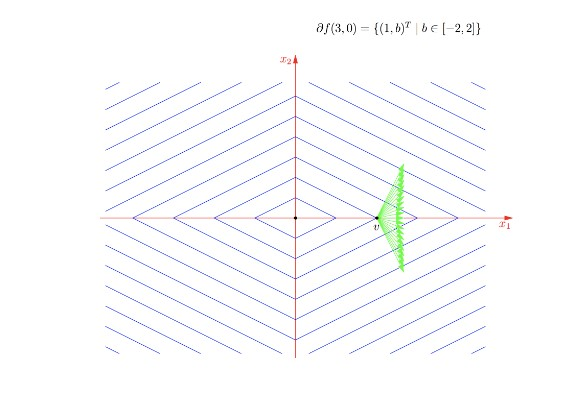
\includegraphics[width=10cm]{lecture_notes/lecture_4/immmages/l4_11.jpg}
\item the substantial is basically just any direction that is strictly towards a decrease in a count plot
\subsection{basic rules for calculating the sub differential }
\item non negative scaling : $ \partial \alphaf(x)=\alpha \partial f(x)\quad \forall \alpha>0$
\item summation $\partial(f(x)+g(x))=d1+d2 \forall d_1\in \partial f(x), d_2\in\partial g(x)$
\item composing with affine functions $\partial f(Ax+b)=A^{t}\partial A^{t}f(Ax+b)$
\item 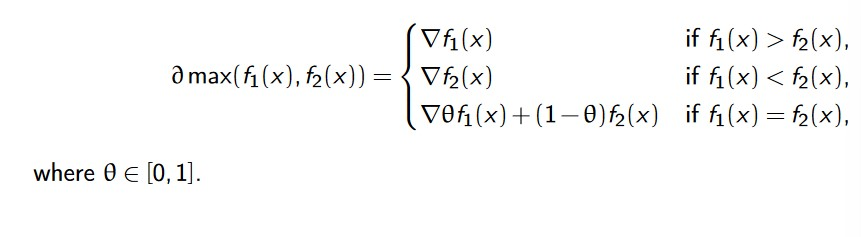
\includegraphics[width=10cm]{lecture_notes/lecture_4/immmages/l4_12.jpg}
\section{sub gradient descent}
\subsection{contour lines and sub gradients}
\item we know that the gradient is the direction of fastest ascent what about the sub gradient?
\item we say that a hyper plane H supports a set S if H intersects S and all of S lies on one side of H, basically H is tangent to S and all points are under or over it 
\item claim if $f:\mathbb{R}^{d}\rightarrow \mathbb{R}$ has a sub gradient g at $x_0$ the hyper lane H orthogonal to h at $x_0$ must support the level set $s=\{x\in \mathbb{R}^{d}|f(x)=f(x_0)\}$
\item proof
\begin{itemize}
    \item for any y we have $f(y)\geq f(x_0)+g^{t}(y_x_0)$ by def of sub gradient 
    \item if y is strictly on the side of h that g points in then g and $(x-x_0)$ are in the same side that is $g^{T}(y-x_0)\geq 0$
    \item $f(y)>f(x_0)$
    \item so y is not in the level set of S
    \item all elements of s must be on H or on the -g side of h.
\end{itemize}
\item the BASIC point is the count of f must lie on one side of the sub gradient 
\item 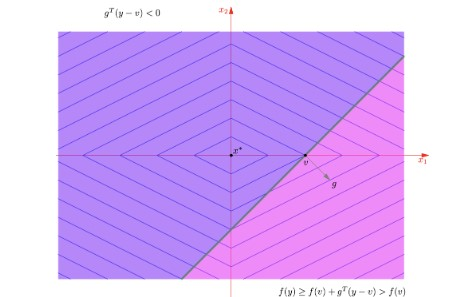
\includegraphics[width=10cm]{lecture_notes/lecture_4/immmages/l4_13.jpg}
\item the points on the side that g points of g will have larger f values than $f(x_0)$ but points in the direction of -g may not have smaller f-vales. so -g may not be a descent direction
\subsection{sub gradient descent}
\item the idea is to move along the sub gradient that is $x\rightarrow x-\alpha g$ where $g\in\partial f(x), \alpha>0$
\item this can increase the objective function, but gets us closer to the minister if f is convex and $\alpha$ is small enough that is $||x_{t+1}-x^{*}||\leq ||x_{t}-x^{*}||$
\item sub gradient do not necessarily converge to zero as we get closer to $x^{*}$ so we need decreasing step sizes 
\item sub gradient methods are slower than gradient descent methods for convex functions 
\item so our svm objective function is $$j(w)=\frac{1}{n}\Sigma_{i=1}^{n}max(0,1-y_iw^{t}x_i)+\lambda||w||^{2}$$
\item we use pegasos algo ie stochastic gradient descent with step size $\alpha=\frac{1}{\lambda t}$
\item algo
\begin{itemize}
    \item initialize $w,t=0,0$
    \item while termination condition not me 
    \item for $j=1...n $ (assume data is randomly shuffled
    \begin{itemize}
        \item t=t+1
        \item $\alpha=\frac{1}{\lambda t}$
        \item if $y^{i}w_{t}^{T}x_i< 1$ $w_{t+1}=(1-\alpha_{t}\lambda)\w_{t}+\alpha_{t}y_{i}x_{i}$
        \item else $W_{t+1}=(1-\alpha_{t}\lambda)w_{t}$
    \end{itemize}
\end{itemize}
\section{dual problem}
\item in addition to solving the problem using sub gradient descent we can solve this problem using a quadratic program 
\item we can study its dual problem to gain insights
\subsection{svm as a quadratic program}
\item the svm problem is given by min $\frac{1}{2}||W||^{2}+\frac{c}{n}\Sigma_{i=1}^{n}\epsilon_{i}$ subject to $\epsilon_{i}\geq 0$ and $\epsilon_{i}\geq (1-yi(w^{t}x_i+b))\quad \forall i$
\item the objective function here is differentiable which is mice
\item we have to learn value for b, d values for $w$ and n for$ \epsilon$ so we have a total of n+d+1 unknowns
\item we have $2n$ affine constraints. (ie they can be expressed as $y=ax+b$
\itme so this is a nice quadratic program 
\subsection{the Lagrangian}
\item general optimization problems with inequality cons taints can be expressed as min $f_{0}(x)$ subject to $f_i(x)\leq 0 $ for $i\in[1,,m]$
\item we can use the Lagrangian to write all this as one problem that we can optimize with out constraints $\mathcal{L}(x,\lambda)=f_{0}(x_i)+\Sigma_{i=1}^{m}\lambda_{i}f_{i}(x) $
\item the $\lambda$'s are called Lagrange multiplies or dual variables they represent how retrieve a certain constraint is
\item so this is a weighted sum of the objective and constraint functions
\subsection{Lagrange dual function}
\item the Lagrange dual function is $$g(\lambda)=inf_{x}\mathcal{L}(x,\lambda)=inf_{x}(f_{0}(x)+\Sigma_{i=1}^{n}\lambda_if_i(x))$$
\item notice here that by taking the infimum we are setting x to a constant and thus $f_{0}(x),f_i(x)$ at each point. meaning that we are really dealing with a linear combination, and linear functions are indeed convex. meaning $g(\lambda)$ is convex
\item the lower bound property tells us if $\lambda\geq 0, g(\lambda)\leq p^{*} $ where p is the optimal value of the optimization problem 
\item so in other words $g(\lambda)$ is a lower bound of of the optimal value of our optimization problem. this does not mean it will always be informative though. 
\subsection{primal and dual problems}
\item for any primal optimization problem minimize $f_{0}(x)$ subject to $f_{i}(x)\leq 0 $ for all $i\in[1,m]$
\item we can write the corresponding Lagrange dual problem as maximize $g(\lambda)$ subject to $\lambda_{i}\geq 0\quad \forall i$
\item the dual problem is always a convex optimization problem. meaning that the objective and inequality constraints are convex, and the equality constraints are affine. 
\item the dual variables often have rel event interpretations 
\item the dual variables proved certificates for optimally
\item 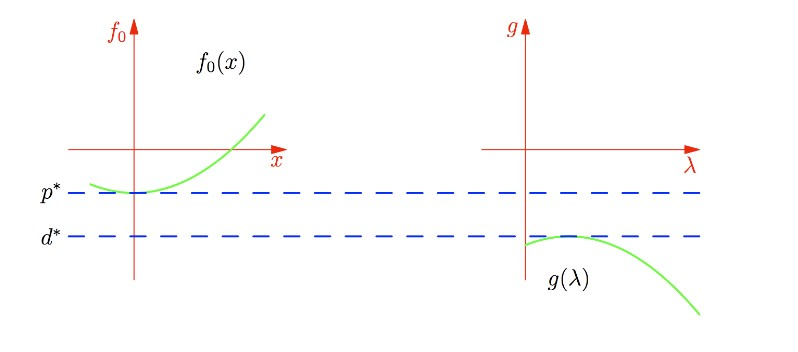
\includegraphics[width=10cm]{lecture_notes/lecture_4/immmages/l4_14.jpg}
\item the above is weak duality meaning that the solution of the dual problem $d^{*}\leq p^{*}$
\item 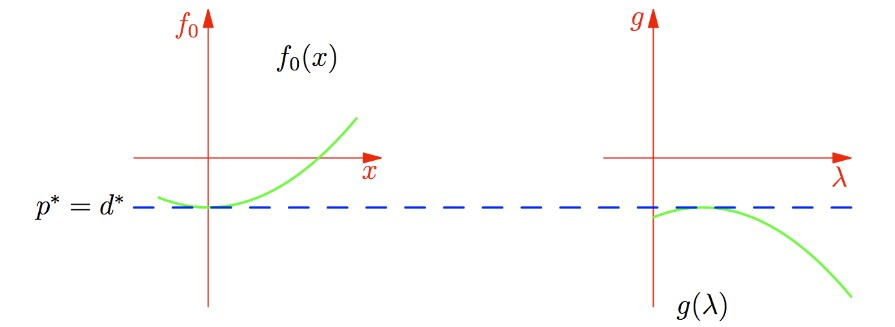
\includegraphics[width=10cm]{lecture_notes/lecture_4/immmages/l4_15.jpg}
\item Strong duality means the solution to the dual problem is equal to the solution to the primal problem 
\item this is pretty common for convex problems 
\subsection{proof of strong duality}
\item assume that we have strong duality and $x^{*}$ is the primal optimal and $\lambda^{*}$ is the dual optimal
\item we know $f_{0}(x^{*})=g(\lambda^{*})=inf_{x}L(x,\lambda^{*})\leq L(x^{*},\lambda^{*})=f_{0}(x^{*})+\Sigma_{i=1}^{n}\lambda_{i}^{*}f_{i}(x^{*})\leq f_{0}(x^{*})$
\item this means $0=\Sigma_{i=1}^{n}\lambda_{i}^{*}f_{i}(x^{*})$ that is we will have strong duality if there is some combination of lambdas and x that result in the sum of all of our constraints at that x times lambda being zero   $0=\Sigma_{i=1}^{n}\lambda_{i}^{*}f_{i}(x^{*})$ 
\item further if we have strong duality then $0=\Sigma_{i=1}^{n}\lambda_{i}^{*}f_{i}(x^{*})$ that means that if $\lambda_{i}>0 $ then $f(x_i)=0$ and if $f(x_i)>0$ then $\lambda_{i}=0$ which is called complementary slackness that is we can either set the constraints it's self to be zero so it does not matter, or optimize the problem such that the lambda on it will be zero so it does not matter
\section{svm dual problem}
\subsection{svm Lagrange multiple rs}
\item
 the svm primal problem is $\frac{1}{2}||W||^{2}+\frac{c}{n}\Sigma_{i=1}^{n}\epsilon_{i}$ subject to $\epsilon_{i}\geq 0$ and $\epsilon_{i}\geq (1-yi(w^{t}x_i+b))\quad \forall i$
 \item so if we let $\lambda_i$ co respond to $-\epsilon_{i}\leq 0$ and $\alpha_{i}$ co respond to 
$(1-y_{i}(W^{t}x_i+b))-\epsilon_{i}\leq 0$
\item then our Lagrangian primal can be written as $$L(w,b,\epsilon, \alpha, \lambda)=\frac{1}{2}||w||_{2}^{2}+\frac{c}{n}\Sigma_{i=1}^{n}\epsilon_i+\Sigma_{i=1}^{n}\alpha_{i}(1-y_i(w^{t}x_i+b)-\epsilon_{i})+\Sigma_{i=1}^{n}\lambda_{i}(\epsilon_{i})$$
\subsection{Strong duality by Slater's}
\item the svm primal problem is $\frac{1}{2}||W||^{2}+\frac{c}{n}\Sigma_{i=1}^{n}\epsilon_{i}$ subject to $\epsilon_{i}\geq 0$ and $\epsilon_{i}\geq (1-yi(w^{t}x_i+b))\quad \forall i$
\item a problem has Strong duality if it meets Slater's constraint qualifications 
\begin{itemize}
    \item the objective is convex and the constrains are affine$ \Rightarrow$ strong duality $\iff$ the problem is feasible (ie has at least 1 point satisfying all constraints)
    \item so for svm we do have strong duality 
\end{itemize}
\subsection{svm first order conditions}
\item the svm dual problem is $g(\alpha. \lambda)=inf_{w,b\epsilon}l(w,b,\epsilon, \alpha, \lambda)=inf_{w,g,\epsilon}[frac{1}{2}||w||_{2}^{2}+\frac{c}{n}\Sigma_{i=1}^{n}\epsilon_i+\Sigma_{i=1}^{n}\alpha_{i}(1-y_i(w^{t}x_i+b)-\epsilon_{i})+\Sigma_{i=1}^{n}\lambda_{i}(\epsilon_{i})]$
\itme then we can take see that $\partial_{w}l=0\rightarrow w=\Sigma_{i=1}^{n}\alpha_{i}y_{I}x_{i}$
\item $\partial_{b}l=0\rightarrow 0=\Sigma_{i=1}^{n}\alpha_{i}y_{i}$
\item $\partial_{\epsilon_{i}}l=0\rightarrow \alpha_{i}+\lambda_{i}=\frac{c}{n}$
\subsection{svm dual function }
\item plugging those condtins back into L we can write 
\item $L=\Sigma_{i=1}^{n}\alpha_{i}-\frac{1}{2}\Sigma_{i=1,j=1}^{n}\alpha_{i}\alpha_jy_iy_jx_j^Tx_i$
\item then the dual function becomes $g=\Sigma_{i=1}^{n}\alpha_{i}-\frac{1}{2}\Sigma_{i=1,j=1}^{n}\alpha_{i}\alpha_jy_iy_jx_j^Tx_i$ if $\Sigma_{i=1}^{n}\alpha_iy+i=0, \alpha_i+\lambda_i=\frac{c}{n}$ and $\-infty$ otherwise 
\item that is if our constraints are not met, we cant use the dual problem to establish a lower bounds 
\item so the dual problem is $sup_{\alpha, \lambda } \Sigma_{i=1}^{n}\alpha_{i}-\frac{1}{2}\Sigma_{i=1,j=1}^{n}\alpha_{i}\alpha_jy_iy_jx_j^Tx_i$ such that $\Sigma_{i=1}^{n}\alpha_iy+i=0, \alpha_i+\lambda_i=\frac{c}{n}$
\subsection{insights form the dual}
\item for convex problems is Slater's condition is satisfied then the kkt conditions prove necessary and sufficient conditions for the optimal solution
\begin{itemize}
    \item there must be primal feasibility ie $f_{i}(x)\leq 0$ for some x and all i 
    \item dual feasibility ie $\lambda \geq 0$
    \item complementary slackness ie $\lambda_{i}f_{i}(x)=0$
    \item and the first order condition must be met $\frac{\partial}{\partial x}l(x,\lambda)=0$
\end{itemize}
\item given $\alpha^{*}$ is the dual solution then by our earlier constraint on w the primal solution is $w^{*}=\Sigma_{i=!}^{n}\alpha_{I}^{*}y_ix_i$
\item c controls the max weight on each example it is kind of like robustness. similar to regularization in the seams that it prevents over fitting to the training data.
\subsection{complementary slackness conditions}
\item recall that $\lambda_{i}$ co responds to the constraint $\epsilon_{i}\leq 0$
\item and $\alpha\_{i}$ co responds to $(1-y_if(x_i))-\epsilon_{i}\leq 0$
\item by our first order condition we know that $\partial_{\epsilon}l=0$ gives us $\lambda_{i}^{*}=\frac{c}{n}-\alpha_{i}^{*}$
\item by Strong duality we must have complementary slackness $(\alpha_{i}^{*}1-y_if(x_i))-\epsilon_{i}^{*}= 0$
\item and $\lambda^{*}\epsilon^{*}=(\frac{c}{n}-\alpha_{I}^*)\epsilon_{i}=0$
\subsection{consequences of complementary slackness }
\item recall that slack variables $\epsilon_{i}=max(0,1-y_i(w^{*t}x_i+b))$ is the hine loss on pair $(X_i,Y_I)$
\item if $y_i(w^{t*}x_i+b)>1$ then the hingle loss for that point is $\epsilon_{i}=0$ and $\alpha_{i}^{*}=0$
\subsection{support vectors}
\item if $\alpha^{*}$ is a sollution ot the dual problem then teh primal sollution is $w^{*}=\Sigma_{i=1}^{n}\alpha^{*}y_ix_i$ with $\alpha^{*}\in [0,\frac{c}{n}]$
\item the $x_i$'s corepsonding to $\alpha_{i}^{*}>0$ these are points where our constraint is active, so that means $(1-y_if(x_i)-\epsilon_{i})=0$ meaning the contraints matter ehre so teh points are either on teh margin or missclafied 
\item so only those points will influince the hyperplane we end up learning 
\item so examples that we miss classfify or few examples on the margin mean we have sparsity in input examples ie only a few points matter 
\end{itemize}
\end{document}
